\chapter{Domain Driven Design}\label{chapter:domain_driven_design}

\section{Introduction}\label{section:domain_driven_design/introduction}
Understanding the problem space can be a very useful way to design software. The common way to understand the problem and communicate them is by using various design models. The design models are the abstraction as well as representation of the problem space. However, when the abstractions are created, there are chances that important concepts or data are ignored or misread. This will highly impact the quality of software produced. The software thus developed may not reflect the real world situation or problem entirely.
\\
Domain Driven Design provides a way to represent the real world problem space so that all the important concepts and data from real world remains intact in the model. The domain model thus captured respects the differences as well as the agreement in the concepts across various parts of the problem space. Moreover, it also provides a way to divide the problem space into manageable independent partitions and makes it easy for developers as well as stakeholders to focus on the area of concern as well as be more agile. Finally, the domain models act as the understandable and common view of the business for both domain experts as well as the developers. This will make sure that the software developed using domain driven design will comply with business need.\cite{Evans:2003aa}\cite{Vernon:2013aa}
\\
There are three basic parts to implement domain driven design:
\begin{enumerate}
\item{Ubiquitous Language}
\item{Strategical Design}
\item{Tactical Design}
\end{enumerate}
\\
However, in order to accomplish the true value of domain driven design, the tactical design is not as compulsory as the first two parts.
\section{Ubiquitous Language}\label{section:domain_driven_design/ubiquitous_language}
Ubiquitous Language is a common language agreed among domain experts and developers in a team. It is important to have a common understanding about the concepts of a business which is being developed and ubiquitous language is the way to assure that. Domain Experts understand the domain in terms of their own jargon and concept. It is difficult for a developer to understand them. Usually, developers translates those jargons into the terms they understand easily during desing and implementation. However along the way of translation, major domain concepts can get lost and the immediate value of the resulting solution might decrease tremendously. In order to prevent creation of such low valued solution, there should be a meet-in-the-middle approach to define common vocabularies and concepts understood by all domain experts as well as the developers. These common vocabularies and concepts make the core of the ubiquitous language.\cite{Evans:2003aa}\cite{Vernon:2013aa}
\\
Along with the common vocabulary and concepts, domain models provide backbone to create ubiquitous language. The models represents not only artifacts but also functionalities, rules and strategies. It is a way to express the common understanding in a visual form providing an easy tool to comprehend.\cite{Evans:2003aa}\cite{Fowler:2006aa} According to \cite{Fowler:2003aa}, domain model should not be confused with data model which represents the business in datacentric view but rather each domain object should contain data as well as logic closely related to the data contained. Domain models are conceptual models rather than software artifacts but can be effectively visualized using \acrshort{UML}.\cite{Scott:2001aa}

\begin{figure}[H]
\begin{center}
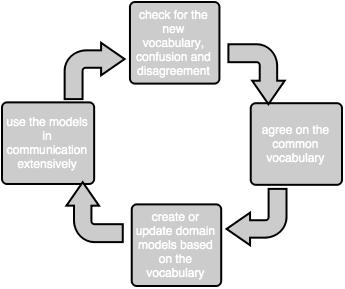
\includegraphics[width=0.8\textwidth]{figures/domain_driven_design_one}
\caption{Process to define Ubiquitous Language \cite{Evans:2003aa}}
\label{fig:domain_driven_design/ubiquitous_language_process}
\end{center}
\end{figure}
\\
The figure \ref{fig:domain_driven_design/ubiquitous_language_process} visualizes the process of discovering the ubiquitous language in any domain. It is not a discretely timed phenomenon but a continous procedure with various phases occuring in a cycle throughout the development cycle.
\\
On arrival of any new term, concept or any confusion, the contextual meaning of those terms are made clear before adding to the domain vocabulary. Next, the vocabularies and concepts are used to create various domain models following \acrshort{UML}. The domain models and various vocabularies for the common laguage among domain experts and developers within the team. It is very important to use only domain vocabularies for communication and understanding which will not only help to reflect the hidden domain concepts in the implementation but also create opportunities to create new vocabularies or refine existing ones in the event of confusion and disagreement.\cite{Evans:2003aa}
\\
Thus, the common vocabulary and domain models form the core of the ubiquitous language and the only way of coming up with the better one is by applying it in communication extensively. Ubiquitous language is not just a collection or documentation of terms but is the approach of communication within a domain.
\\
\section{Strategical Design}\label{section:domain_driven_design/strategical_design}
When applying model-driven approach to an entire enterprise, the domain models get too large and complicated. It becomes difficult to analyse and understand all at once. Furthermore, it gets worse as the system gets bigger. The strategical design provides a way to divide the entire domain models into small,manageable and interoperable parts which can work together with low dependency in order to reflect the functionalities of the entire domain. The goal is to divide the system into modular parts which can be easily integrated. Additionally, the all-cohesive unified domain models of the entire enterprise cannot reflect differences in contextual vocabularies and concepts.\cite{Fowler:2014ab}\cite{Evans:2003aa}\cite{Vernon:2013aa}
The strategical design specifies three major steps.
\\
\begin{shaded}Step 1: Divide problem domain into subdomains \end{shaded}
\\
The domain represents the problem being solved by the software. The domain can be divided into various sub-domains based on the organizational structure of the enterprise, each sub-domain responsible for certain area of the problem. The \cite{Engels:2015aa} provides a comprehensive set of steps to identify sub-domains.
\begin{enumerate}
\item \textbf{Identify core business functionalities and map them into domain:} \\
A core business functionality represents the direct business capability which holds high importance and should be provided by the enterprise in order for it to succeed. For example, for any general e-commerce enterprise, the core focus will on the high amount orders being received from the customers and maintain the inventory to fulfil the orders. So, for those kind of e-commerce enterprises, 'Order Management' and 'Inventory Management' will be the some of the core domains.
\\
\item \textbf{Identify generic and supporting subdomains:} \\
The business capabilities which are viable for the success of business but not represent the specialization of the enterprise falls into supporting subdomains. The supporting subdomain does not require the enterprise to excel in these areas. Additionally, if the functionalities are not specific to the business but in a way support the business functionalities, then these are covered by generic subdomains. For example: for an e-commerce enterprise, 'Payment Management' can be a supporting subdomain whereas 'Reporting' and 'Authentication' can be generic subdomains.\cite{Vernon:2013aa}
\\
\item \textbf{Divide existing subdomains having multiple independent strategies:}\\
The subdomains found from earlier steps are analyzed to check if there are mutually independent straties to handle the same functionality. The subdomain can then be further divided into multiple subdomains along the dimension of strategies. For example: the 'Payment Managment' subdomain discovered in earlier step can have different way of handling online payment depending upon the provider such as bank or paypal etc. In that case 'Payment Management' can be further divided into 'Bank Payment Management' and 'Paypal Payment Management'.
\end{enumerate}
\\
\begin{shaded}Step 2: Indentify bounded contexts\end{shaded}
\\
\begin{shaded}Step 3: Discover relationship among bounded contexts using Context Map\end{shaded}